\chapter{Resultados}

\section{Evaluación de nuestra implementación}

En este momento vamos a evaluar debilidades y fortalezas de nuestra implementación de ext2. 

La debilidad obvia, y que no nos importa, es que la implementación no es completa: carece de manejo de permisos de archivos, cosa que no nos importa en DeliriOS.

Además, es mucho más simple que la implementación de ext2 de otros sistemas operativos como Linux, y usa algoritmos mucho menos sofisticados. Sin embargo, no esperaremos que su performance sea mucho peor. Esto lo veremos más adelante.

Una métrica no siempre utilizada al comparar varias implementaciones de una misma especificación es su simplicidad. Aquí sí lo haremos, dado que DeliriOS es un sistema operativo que se concentra en ser minimal, aunque funcional.

Comparemos la cantidad de líneas de código de cada implementación.

\begin{figure}[H]
  \centering
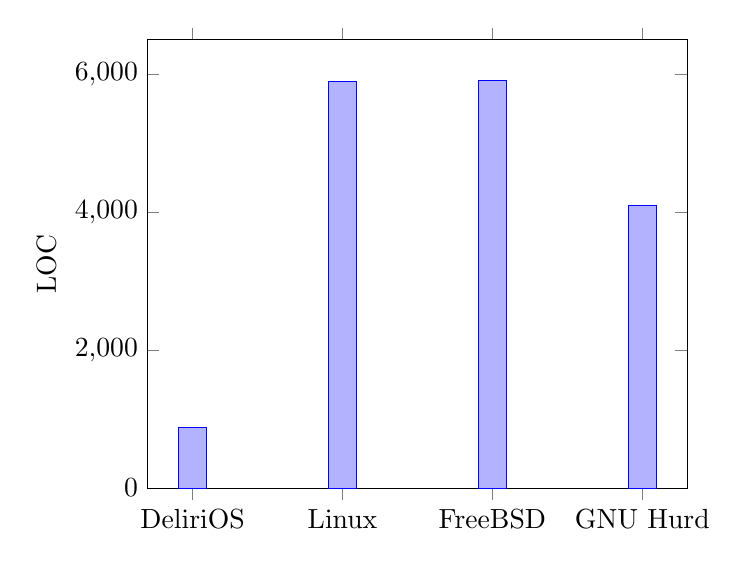
\begin{tikzpicture}
\begin{axis}[
	%x tick label style={/pgf/number format/1000 sep=},
  symbolic x coords={DeliriOS, Linux, FreeBSD, GNU Hurd},
	ylabel=LOC,
  xtick=data,
  ymin=0,
	ybar,
]
\addplot 
	coordinates {
    (DeliriOS,876)
    (Linux,5899)
    (FreeBSD,5910)
    (GNU Hurd,4104)};
\end{axis}
\end{tikzpicture}
\caption{Líneas de código de la implementación de ext2 de cada sistema operativo. El programa \texttt{cloc} fue utilizado para medirlas, dado que cuenta las lineas de código puro, sin contar líneas vacías y de comentarios.}
\end{figure}

\begin{figure}[H]
  \centering
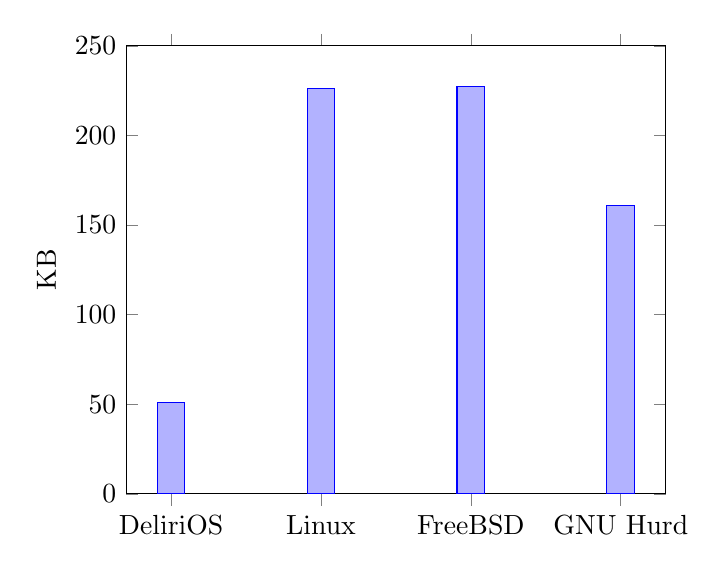
\begin{tikzpicture}
\begin{axis}[
	%x tick label style={/pgf/number format/1000 sep=},
  symbolic x coords={DeliriOS, Linux, FreeBSD, GNU Hurd},
	ylabel=KB,
  xtick=data, 
  ymin=0,
	ybar,
]

%(DeliriOS,52477)
%(Linux,231427)
%(FreeBSD,232832)
%(GNUHurd,164757)};
\addplot 
	coordinates {
    (DeliriOS,51.24)
    (Linux,226.00)
    (FreeBSD,227.37)
    (GNU Hurd,160.89)};
\end{axis}
\end{tikzpicture}
\caption{Tamaño del código fuente de la implementación de ext2 de cada sistema operativo.}
\end{figure}


Como puede verse, la implementación de DeliriOS es realmente simple y corta. Esto es muy bueno, dado que por un lado es más fácil de entender para alguien que se acople al proyecto, y por otro lado permite que el binario de DeliriOS siga siendo diminuto (entra entero en la cache L1 de código de un core de un procesador moderno).



\section{Performance de nuestra implementación}

Para medir la performance de nuestra implementación decidimos compararla con la de Linux.
Tenemos que aclarar que medir este tipo de piezas de software y compararlas es muy difícil por varias razones.
Por ejemplo, como son operaciones dentro de todo muy rápidas, por lo que si las mediciones están mal hechas, el \emph{preemption} del sistema operativo las puede arruinar.

Como DeliriOS sólo soporta ATA PIO por ahora, necesitamos algún ambiente de prueba en el que esto no sea un limitante. Por eso, testeamos sobre una máquina virtual que emulara este tipo de disco.

Las mediciones las tomamos de la siguiente manera: linkeamos los mismos tests que los tests de correctitud por fuera de delirios y los usamos para testear distintas operaciones sobre una imagen de disco.
Tambi\'en realizamos las mismas operaciones con Linux.
Esto ya es un problema, porque el código de DeliriOS va a correr en \emph{userspace}, mientras que el código de Linux va a correr en \emph{kernelspace}.
Veremos cómo corregir esto más adelante, pero primero veamos cómo testeamos. Realizamos 500 repeticiones de cada test, y cada test consistió en lo siguiente.

\begin{itemize}
    \item[create] 36 archivos creados.
    \item[mkdir] 10 directorios creados.
    \item[read] 104000 caract\'eres leídos de 2 archivos.
    \item[remove] 8 archivos borrados.
    \item[write] 104000 caract\'eres escritos en 2 archivos.
\end{itemize}

Todos los tests fueron corridos con el correspondiente flush a disco (fsync en Linux) de tal manera que sean efectivos. Además, con DeliriOS medimos el tiempo de acceso a disco, y se lo restamos a ambas mediciones. Es decir, los tiempos que veremos no son los tiempos totales, si no los tiempos totales sin los tiempos que el programa se pasa leyendo o escribiendo el disco.

Veamos los resultados.


\begin{figure}[H]
  \centering
  \begin{minipage}[b]{0.49\textwidth}
    \includegraphics[width=\textwidth]{tiempos/create.pdf}
    \caption{}
  \end{minipage}
  \begin{minipage}[b]{0.49\textwidth}
    \includegraphics[width=\textwidth]{tiempos/mkdir.pdf}
    \caption{}
  \end{minipage}
  \hfill
\end{figure}
\begin{figure}[H]
  \centering
  \begin{minipage}[b]{0.49\textwidth}
    \includegraphics[width=\textwidth]{tiempos/read.pdf}
    \caption{}
  \end{minipage}
  \begin{minipage}[b]{0.49\textwidth}
    \includegraphics[width=\textwidth]{tiempos/remove.pdf}
    \caption{}
  \end{minipage}
\end{figure}
\begin{figure}[H]
  \centering
  \includegraphics[width=0.5\textwidth]{tiempos/write.pdf}
  \caption{}
\end{figure}

Como se ve, Linux es múcho más rápido en la mayoría de las funciones, excepto en remove. Creemos que la diferencia en remove se debe a que remove es una operación extremadamente barata, y Linux tiene muchas estructuras que debe mantener en cache (como índices), entonces actualizarlas le lleva la diferencia de tiempo que se ve.

Sin embargo, como dijimos antes, los tests están lejos de ser exactos, dado que DeliriOS corre en \emph{userspace} pero Linux corre en \emph{kernelspace}. Pero, como se puede ver en \cite{Rajgarhia:2010:PEU:1774088.1774130}, un trabajo muy extenso que analiza diferencias de performance entre filesystems que corren en el \emph{kernelspace} vs. en el \emph{userspace}, la diferencia llega a ser de 600\% de pérdida de performance.

Hacer la experimentación en DeliriOS nativo no es lo mejor para este tipo de experimentos, porque el clock con el que medimos los tiempos no tiene la granularidad suficiente.
Esto se debe a que usamos el RTC (Real Time Clock), que tiene una granularidad máxima de 122 us.
Por esta razón, solo corrimos el test más exigente, que es el de escritura. Este test, al igual que el anterior, es el tiempo de corrida total, menos el tiempo de acceso a disco.
Veamos los resultados.

\begin{figure}[H]
  \centering
  \includegraphics[width=0.5\textwidth]{tiempos/delirios_linux.pdf}
  \caption{Tiempos en DeliriOS vs. Linux en la prueba de escritura. Cada uno fue corrido en una máquina virtual de iguales condiciones, y a cada tiempo se le restó el tiempo de acceso a disco medido en cada caso. En el caso de Linux, medimos el tiempo de acceso a disco con delirios corriendo sobre Linux, como explicamos antes.}
\end{figure}

Las diferencias de performance ahora son mucho más razonables, dado que el código de DeliriOS es mucho más simple. Sin embargo, obviamente el código de Linux es mucho mas sofisticado, y funciona mejor seguramente en discos más llenos, por ejemplo, dado que sus algoritmos de reserva de bloques son mucho más complejos.

La varianza de Delirios es mucho mas alta, dado que la granularidad es muy baja, por lo que explicamos anteriormente.

